\documentclass[11pt]{article}
\usepackage{graphicx}
\usepackage{fullpage}
\usepackage{anysize}
\usepackage{caption}
\usepackage{titlesec}
\usepackage[usenames,dvipsnames, x11names]{xcolor} % load xcolor and make it recognise the names... 
\usepackage{colortbl}
\usepackage{color, soul} %the soul package allows you to hilight text with \hl{}
\usepackage{hyperref}   % this creates hyperlinks for figure and table referencing (and all other referencing too!)
\usepackage{csvsimple}
\usepackage{tablefootnote}
\usepackage{floatrow}  % to hepl place table captions
\usepackage[hang,flushmargin]{footmisc} %The 'hang' option flushes the footnote marker to the left margin of the page, while the 'flushmargin' option flushes the text as well
\usepackage{lipsum} % these two are required to get good table footnotes
\usepackage{threeparttable}
\usepackage{tikz}
\usepackage{longtable}
\usepackage{gensymb}
%%%%%%%%%%%%%%%%%%%%%%%%%
% Defining format for hyperlinks 
\hypersetup{colorlinks, % left blank (no == to) so no red square
linkcolor= PineGreen, 
filecolor= TealBlue, 
urlcolor= PineGreen,
citecolor= NavyBlue}
\RequirePackage[margin=1in]{geometry} % customize margins 
\RequirePackage{pdflscape}
% this bit sets the section formatting
\titleformat{\section}
  {\normalfont\sffamily\Large\bfseries\color{CornflowerBlue}}
  {\thesection}{1em}{}
% this bit sets the caption formatting formatting
\usepackage[font={bf,small}]{caption}
% to get the table captions at the top of the table
\floatsetup[table]{capposition=top}
% remove the paragraph indenting 
%\setlength{\parindent}{0pt}
\setlength{\parskip}{1em}
\newcommand{\spper}{\hspace{0.5mm}\%}
\newcommand{\spkg}{\hspace{0.5mm}kg}
\newcommand{\spmt}{\hspace{0.5mm}mt}

%________________________________________________
% Change this to the path of the individual country
% \newcommand{\CntPath}{C:/Longline_Reports/Plots/TO}
% \newcommand{\GenPath}{C:/Longline_Reports/Plots}
% \newcommand{\CntLb}{TO}
%________________________________________________


\usepackage{Sweave}
\begin{document}
\Sconcordance{concordance:WHATapp_Report.tex:WHATapp_Report.Rnw:%
1 51 1 1 0 3 1 1 7 292 1}


% grab my numbers and tables created in R

% make the cover page
\pagenumbering{gobble} % switch off page numbering
\makeatletter
\def\parsecomma#1,#2\endparsecomma{\def\page@x{#1}\def\page@y{#2}}
\tikzdeclarecoordinatesystem{page}{
    \parsecomma#1\endparsecomma
    \pgfpointanchor{current page}{north east}
    % Save the upper right corner
    \pgf@xc=\pgf@x%
    \pgf@yc=\pgf@y%
    % save the lower left corner
    \pgfpointanchor{current page}{south west}
    \pgf@xb=\pgf@x%
    \pgf@yb=\pgf@y%
    % Transform to the correct placement
    \pgfmathparse{(\pgf@xc-\pgf@xb)/2.*\page@x+(\pgf@xc+\pgf@xb)/2.}
    \expandafter\pgf@x\expandafter=\pgfmathresult pt
    \pgfmathparse{(\pgf@yc-\pgf@yb)/2.*\page@y+(\pgf@yc+\pgf@yb)/2.}
    \expandafter\pgf@y\expandafter=\pgfmathresult pt
}
\makeatother

\begin{tikzpicture} [remember picture, overlay,every node/.style={anchor=center}] {               
\node  at (page cs:0,0.8) {                                % [anchor=\bound]

\includegraphics [width=22cm]{C:/GitHub/WHATapp/Writing/flag_logos/banner_new.png}};
\node  at (page cs:0,0.3) [blue]{ 
{{\huge{\bfseries An introduction to the WHATapp tool for}}}};
\node  at (page cs:0,0.23) [blue]{ 
{{\huge{\bfseries visualising high seas allocations}}}};
\node  at (page cs:0,-0.05) {

\includegraphics [width= 3in]{C:/GitHub/WHATapp/Writing/flag_logos/FFA.png}};
\node  at (page cs:0,-0.6) {

\includegraphics [width= 1in]{C:/GitHub/WHATapp/Writing/flag_logos/NZ_aid_logo.png}};
\node  at (page cs:0,-0.4) {
{\Large This report was funded by the New Zealand Aid Progamme.}};
\node  at (page cs:0,-0.8) [blue]{ 
{Issue Specific National Report, (An introduction to WHATapp for visualising allocations) {\bf XXXX 2019} }};
\node  at (page cs:0,-0.85) [blue]{ 
{\small Please address inquiries to: Sam McKechnie (samm@spc.int)  }};
\draw [thick] [blue] (page cs:-1,-0.75) rectangle (page cs:1,-0.75);
     }
\end{tikzpicture}
\clearpage     % goes to new page but progresses all floating figures up to that point 
%\restoregeometry

\pagenumbering{arabic}  % start the page numbering again
\section{Introduction} \label{sec:intro}
The establishment of hard limits and allocations for the high seas were addressed in CMM 2017-01 with decision making scheduled for the 2019 commission meeting. In preparation, FFA members have conducted a series of workshops to develop criteria and a strategy for approaching the allocation process. These have highlighted the complexity of the issues involved, the large number of potential criteria that may be considered, the diverse approaches taken by other tuna RFMOs and similar bodies, and the potentially conflicting rankings that different CCMs in the WCPFC will give to different criteria.

Although there are difficulties in identifying and sometimes formulating criteria, what is clear is the need for members to have a means of visualising allocations under different scenarios. This is particularly the case when allocations are based on multiple criteria each of which may be given different weightings when calculating allocation values. Initial tools to this end were constructed in excel and have recently been extended to `Shiny' - software based on the R statistical language that allows the construction of interactive web-based apps. This report is intended to be a support document for the app that demonstrates how to install and run the app, the range of features that can be modified, and explicitely outlines the calculations behind the scenarios included.

The app is simply a tool to visualise the criteria (and their weightings) and the difficulties associated with the allocation process therefore tend to be centred around the selection and formulation of the criteria rather than the developement of the app itself. For example, some criteria such as economic dependency are difficult to define and synthesise into discrete values for each CCM. The set of criteria included in the app and the methods to weight them should not therefore be considered a final set or an accepted methodology and we will continue to develop the app to suit the needs of the membership as further criteria are suggested or existing criteria are modified.



\section{Running the app}
Shiny apps typically run via a local server or are web-based which requires users to have the R software (and applicable packages) installed, and in the case of the latter, a reliable internet connection. These are both barriers to easy distribution of an app, for example at workshops - particularly in the Pacific where internet connectivity can be limited.

We have therefore developed a fully portable version of the app that does not require internet access, or the installation of R and knowlege of its use. The downside of this approach is that a web browser and a portable version of R must be packaged together with the usual components of the app. This leads to a relatively large file size, although  no true `installation' is necessary and so deletion of the app after use is simple. At this stage it is also restricted to windows operating systems. 

The first step in using the app is to download the zipped file from the web or copy it from an external harddrive. This should be unzipped to where you want to store and run the app from. It is recommended to unzip the file to somewhere other than the `downloads' folder as it may be difficult to run a .bat or .vbs from this location. Now click into the WHATapp folder and you should see a file structure very similar to that shown in Fig. \ref{fig:expl1screen}. Running the app is a simple matter of double clicking run.vbs as a first choice, or alternatively run.bat (both circled in Fig. \ref{fig:expl1screen}). Note that if utilising the run.bat option you must not only close the app window but also close the black command prompt window (Fig. \ref{fig:batscreen}) to completely terminate the app after you have finished using the app.

Depending on your machines security settings you may encounter a warning popup window the first time you double click the run.vbs or run.bat. {\bf Click XXXX.}. Alternatively, try right clicking the run.vbs or run.bat and selecting `Run as administrtor'. With any luck the app will successfully launch after a few seconds and you should see a screen similar to Fig. \ref{fig:frontpg}. If the formatting of the browser window is messy then it should be possible to adjust this by zooming in (press `ctrl' and `+') or out (press `ctrl' and `-').

 \begin{figure} [h]
  \centering
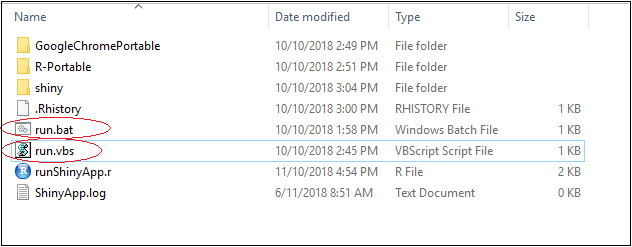
\includegraphics[width=1\textwidth]{C:/GitHub/WHATapp/Writing/Explorer_Folder_1.png}
  \caption {The cmd.exe screen that must be closed when exiting WHATapp when running via the run.bat option.}
  \label{fig:expl1screen}
\end{figure}



 \begin{figure} [h]
  \centering
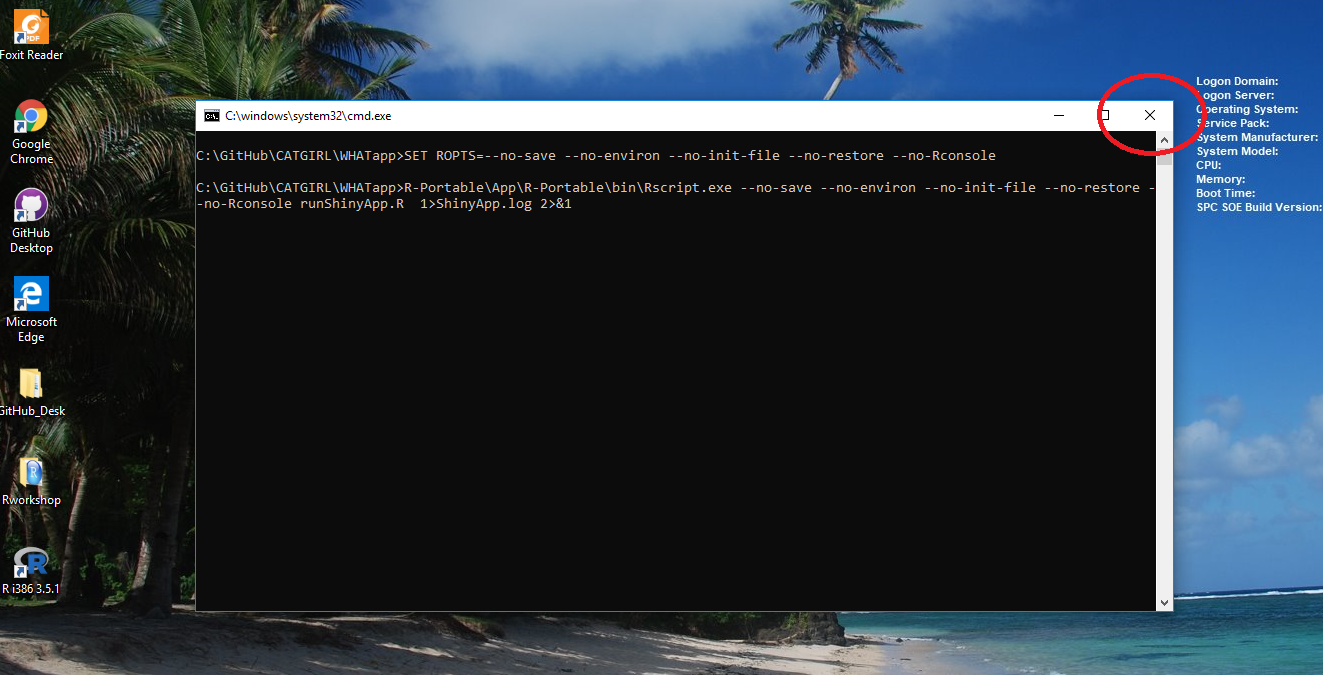
\includegraphics[width=1\textwidth]{C:/GitHub/WHATapp/Writing/Bat_Screenshot.png}
  \caption {The cmd.exe screen that must be closed when exiting WHATapp when running via the run.bat option.}
  \label{fig:batscreen}
\end{figure}


 \begin{figure} [h]
  \centering
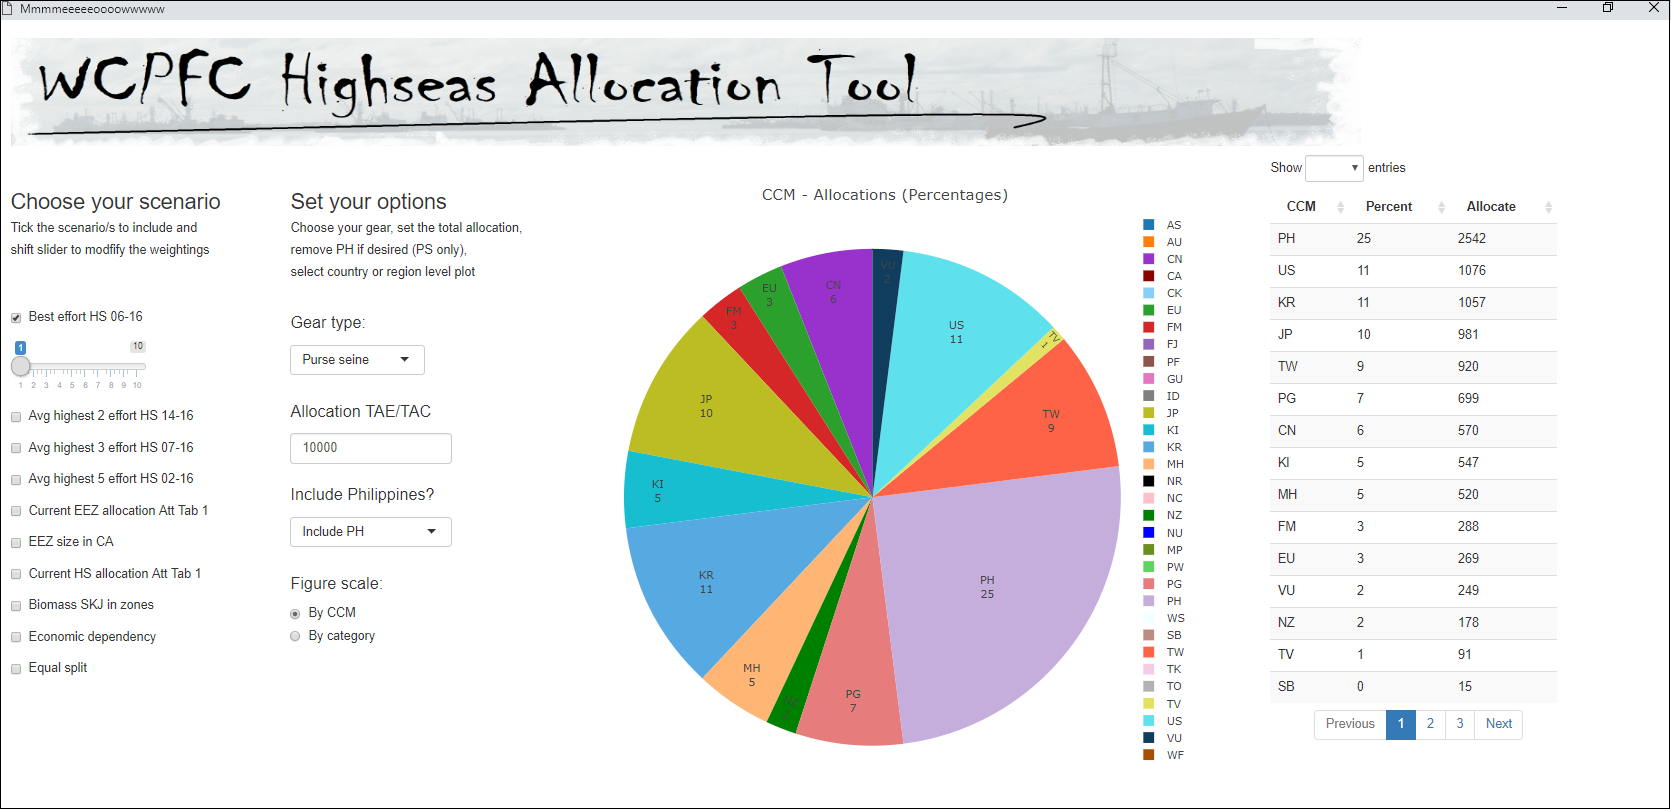
\includegraphics[width=1\textwidth]{C:/GitHub/WHATapp/Writing/App_Front_Page.png}
  \caption {The cmd.exe screen that must be closed when exiting WHATapp when running via the run.bat option.}
  \label{fig:frontpg}
\end{figure}


 \begin{figure} [h]
  \centering
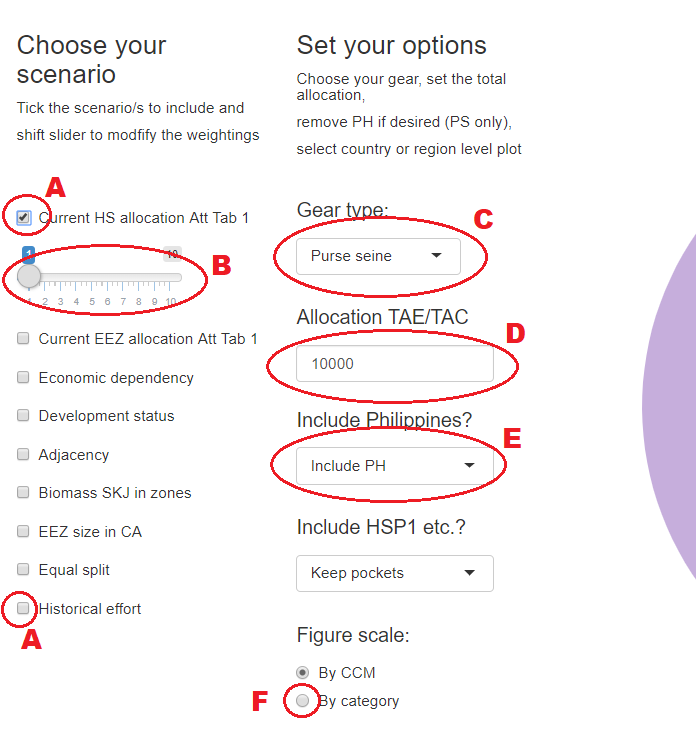
\includegraphics[width=0.8\textwidth]{C:/GitHub/WHATapp/Writing/Features_Fig.png}
  \caption {The cmd.exe screen that must be closed when exiting WHATapp when running via the run.bat option.}
  \label{fig:featpg}
\end{figure}




\section{Features of the app}

\subsection{Controlling the scenarios}
Once the app is running you will see two columns of text and features on the left hand side of the dashboard (Fig. \ref{fig:featpg}). These control the scenarios that you can investigate and also some other features of the plots and tables that show the resulting allocations. To control the app you can modify the following:
\begin{itemize}
\item The left-most column (under `Choose your scenario') shows each of the {\bf X} criteria that can be selected and multiple scenarios can be selected simultaneously by simply clicking the appropriate check boxes (see letter {\bf A}). Further details of each sceario are presented in section \ref{sec:scendet} and the remainder of this section outlines the control of the settings.
\item Once a check box is selected and a tick appears, a slider bar will also be activated for that criteria ({\bf B}). The slider bar sets the weighting of that particular criteria with values between 1 and 10 being allowable. If only one tick box is checked then moving the slider will not impact the allocation at all (the plot and table will not change). However, if multiple boxes are ticked then the sliders determine how much weight is given to each criteria. For example, if the first two boxes are ticked and the slider for criteria 1 is set at 1, and for criteria 2 it is set at at 3, then the latter will have 3 times the weighting of the former. If the slider bar for each criteria is set at 1 then they will all have the same weighting.
\item The second column of widgets defines other (than critera) features of the app to be considered. The drop down menu ({\bf C}) allows switching between the purse seine and longline allocations. Note that there are different criteria present for the two gear types.
\item The box shown by {\bf D} defines the total allowable effort (TAE; in days) and total allowable catch (TAC; in metric tonnes), for purse seine and longline respectively, from which the allocations are made. The value can be modified by clicking on the box and typing in the desired value. This number represents the total catch or effort on the high seas that must be decided before individual CCMs can be allocated specific quantities.
\item Under the purse seine scenarios there is a drop down menu that allows allocations to be made either including or excluding the Philippines (PH). The option to exclude PH is in response to the unique nature of this fleet on the high seas: they have special conditions under the CMM; are predominantly operating in high seas pocket 1; they have very low CPUE and are operationally very different from other fleets; and they have a very high effort that can dominate the effort allocations when based on historical effort criteria. For these reasons, it may be neccessary for this fleet to be treated differently during allocations, and its presence in the app can obscure patterns of allocations among the remaining CCMs under certain condtions. Consequently, the user can decide if this fleet should be excluded from the visualisations or not.
\item Also under the purse seine scenerios there is a further drop down menu that allows the user to either include or exclude several high seas pockets from the historical catch scenarios. The reason for this option is that several high seas pockets (e.g. HSP1; Fig. {\bf X}) were effectively closed to fishing by the CMM around {\bf 2009}.
\item The final option allows the user to switch between viewing the allocations by individual CCMs or by subregional groupings by clicking on the desired button. These groupings are distant water fishing nations (DWFN), FFA members that also belong to the PNA (FFA-PNA), other FFA members (FFA-OTH), Indonesia and Philipines (IDPH) and other CCMs that do not belong to any of these categories (OTH; for example New Caledonia and French Polynesia).
\end{itemize}


\subsection{Summaries of resulting allocations}
Once a certain scenario has been set and the criteria for the allocations chosen, then the app will automatically update and display the allocations for each CCM or sub regional group, with the main features illustrated in Fig. \ref{fig:outputpic}. The allocations are displayed in the form of a pie chart with the CCM/group and the proportional allocation (in percentage form - see {\bf A} in the figure) - by hovering over a pie segment the values for that CCM/group will be displayed in more detail. The chart only shows the proportional allocation and so a table is also displayed that restates the percentage allocated ({\bf B} in the figure) but also allocates the TAE/TAC into absolute allocations ({\bf C}) to the indivicual CCMs/groups in days (purse seine) and metric tonnes of catch (longline). Note that the format of the table is also interactive with the number of entries user-defined by the drop down box ({\bf D}) and their order can be changed by clicking on the bold table headers (e.g. `{\bf Allocate}'; {\bf C}). If the entry in {\bf D} is left blank and not all CCMs are displayed, the `pages' indicated by {\bf E} can be scrolled through to find a particular CCM.



 \begin{figure} [h]
  \centering
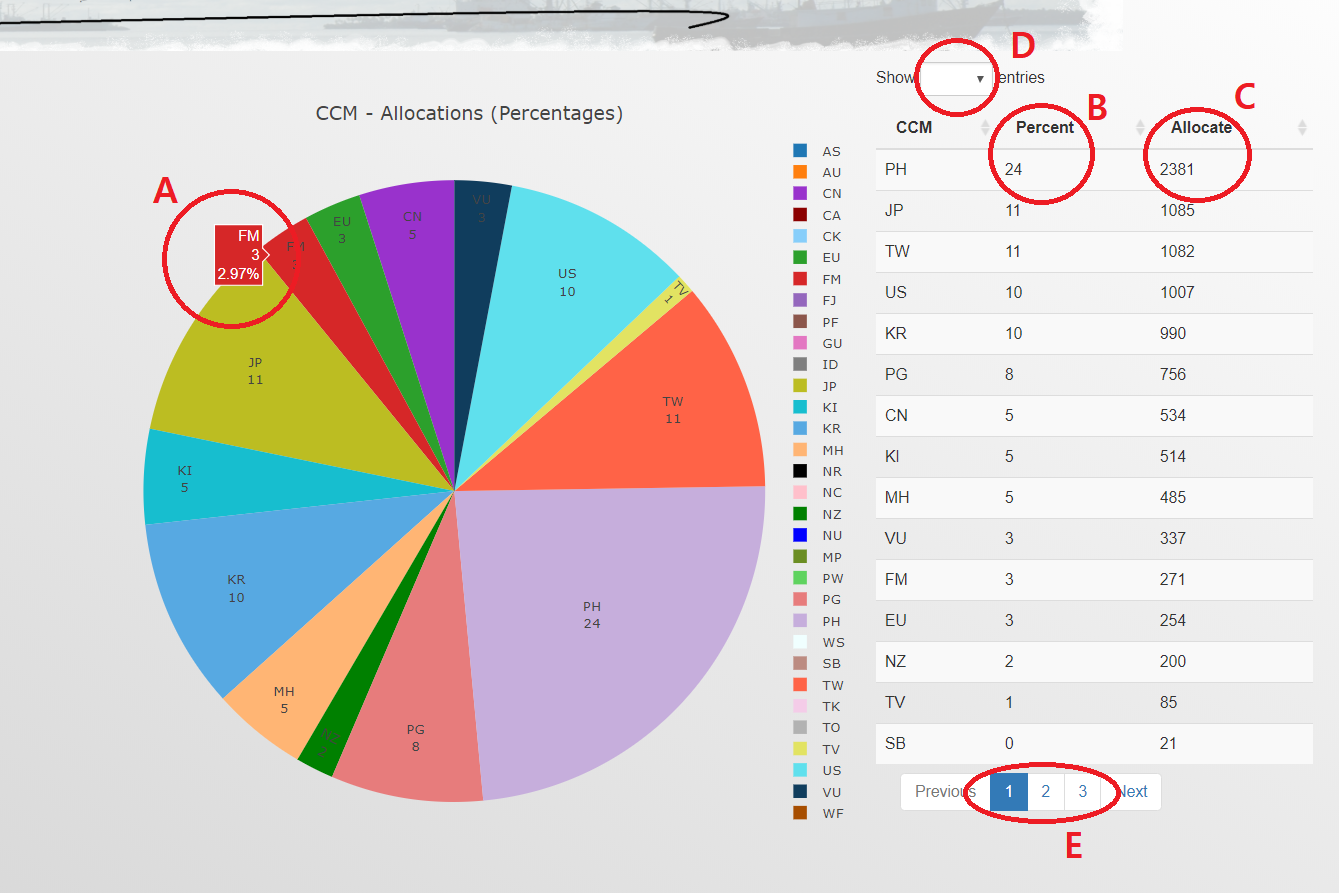
\includegraphics[width=0.8\textwidth]{C:/GitHub/WHATapp/Writing/Output_Figure.png}
  \caption {A picture of part of the app dashboard showing some of the features of the allocation ouput.}
  \label{fig:outputpic}
\end{figure}


\section{Calculation of values for each criteria} \label{sec:scendet}
This section details the calculations and definitions used to determine the values used for each CCM for each criteria. 

\subsection{Criteria for purse seine scenarios}

\subsubsection*{Current high seas limits}
Some CCMs already have purse seine effort limits on the high seas. This criteria uses the values for CCMs that are outlined in table 2 of CMM 2017-01 Attachment 1 and all CCMs not specified in that table receive zero values.

\subsubsection*{Current EEZ limits}
Many CCMs have purse seine effort limits within their EEZs and these are outlined in table 1 of CMM 2017-01 Attachment 1. These values are used for all applicable CCMs with the values used for individual PNA members {\bf based on...} The EEZ limits for Australia, New Caledonia and New Zealand are catch-based and these were converted to effort limits by calculating the mean CPUE for the three EEZs over the period {\bf XXXX-XXXX} and dividing the catch value in the table by the appropriate CPUE to give an equivalent effort-based limit. All CCMs not specified in that table receive zero values for this criteria.

\subsubsection*{Biomass of skipjack in EEZs}

\subsubsection*{Economic dependency}

\subsubsection*{EEZ size}
The area of EEZ in the WCPFC convention area between 20\degree N and 20\degree S, {\bf excluding land area and archipelagic waters}.

\subsubsection*{Equal split}
Very simply, this criteria allocates over all CCMs equally.

\subsubsection*{Catch in adjacent zones} 


\subsubsection*{Historical effort}
This criteria allocates more of the TAE to a CCM if it has a history of fishing in the high seas. The user has additional choices available in the app for this criteria related to the timing of the calculations of historical effort. Initially the annual effort fished by each CCM in the high seas between 20\degree N and 20\degree S, for the period 2002--{\bf 2016} was extracted from the databases. When the tick box for this criteria is checked three widgets will appear - the usual criteria weighting bar, but also an additional sliding bar and a numeric box which together determine the timing and methods of calculating historical effort.



\section{General discussion}

The purpose of the software and this report is to make the visualisation of potential allocation scenarios easily accessible to members. To this end we welcome feedback on how the app could be improved. This may include improvements in the presentation of results or the instructions of how the app is to be used.



\newpage

%\input{C:/NZ_Seabirds/Plots/EffDistCK.tex}


%  \begin{figure} [h]
%   \centering
% \includegraphics[width=1\textwidth]{\CntPath/ACE_bySpp_with_effort.png}
%   \caption {Annual catch estimates (lower panels) in 1,000's mt for the four main tunas and the `other' (bycatch) category since 1990. The upper two panels display the effort since 2000 (when logsheet data became more numerous) in number of sets (purple; 1,000's of sets) and number of hooks (blue; millions of hooks) which are calculated by raising the logsheet data based on the annual catch estimates.}
%   \label{fig:lab1}
% \end{figure}
% 
% \newpage
% 
%  \begin{figure} [h]
%   \centering
% \includegraphics[width=1\textwidth]{\GenPath/Map_ALBll_Full-ALB-CPUE_mon-1.png}
%   \caption {Have a meeting lined up with Peter about what can and cant be presented along these lines.}
%   \label{fig:lab2}
% \end{figure}
% 
% 
% \newpage
% 
%  \begin{figure} [h]
%   \centering
% \includegraphics[width=1\textwidth]{\CntPath/ACE_CountryComp_Composite_ALB_raw_shown.png}
%   \caption {Comparison of annual catch (metric tonnes) of albacore within the EEZs of {\bf 17} South Pacific countries. The large upper panel shows the average catch in each EEZ over the period 2010--2017, and the rankings among countries, while the lower panels show this same information for each year separately. Your EEZ is indicated by the coloured bars.}
%   \label{fig:ACErelalb1}
% \end{figure}
% 
% \newpage
% 
%  \begin{figure} [h]
%   \centering
% \includegraphics[width=1\textwidth]{\CntPath/ACE_CountryComp_Composite_ALB_density_shown.png}
%   \caption {Comparison of the density of annual catch of albacore (metric tonnes per km$^2$ within the EEZs of {\bf 17} South Pacific countries. The large upper panel shows the average density of catch in each EEZ over the period 2010--2017, and the rankings among countries, while the lower panels show this same information for each year separately. Your EEZ is indicated by the coloured bars.}
%   \label{fig:ACErelalb2}
% \end{figure}
% 
% \newpage
% 
%  \begin{figure} [h]
%   \centering
% \includegraphics[width=1\textwidth]{\CntPath/ACE_CountryComp_Composite_BET_density_shown.png}
%   \caption {Comparison of the density of annual catch of bigeye (metric tonnes per km$^2$ within the EEZs of {\bf 17} South Pacific countries. The large upper panel shows the average density of catch in each EEZ over the period 2010--2017, and the rankings among countries, while the lower panels show this same information for each year separately. Your EEZ is indicated by the coloured bars.}
%   \label{fig:ACErelbet}
% \end{figure}
% 
% \newpage
% 
%  \begin{figure} [h]
%   \centering
% \includegraphics[width=1\textwidth]{\CntPath/ACE_CountryComp_Composite_YFT_density_shown.png}
%   \caption {Comparison of the density of annual catch of yellowfin (metric tonnes per km$^2$ within the EEZs of {\bf 17} South Pacific countries. The large upper panel shows the average density of catch in each EEZ over the period 2010--2017, and the rankings among countries, while the lower panels show this same information for each year separately. Your EEZ is indicated by the coloured bars.}
%   \label{fig:ACErelyft}
% \end{figure}
% 
% \newpage
% 
% 
%  \begin{figure} [h]
%   \centering
% \includegraphics[width=1\textwidth]{\CntPath/CPUE_Trends_Both.png}
%   \caption {Fluctuations in the CPUE of albacore tuna in your EEZ. The top figure shows the CPUE at the monthly scale and the bottom figure shows it at the annual scale. The black lines are the nominal CPUE (the raw observed CPUE) while the blue lines are the standardised CPUE which are hoped to better reflect the underlying biomass of albacore in the EEZ over time.}
%   \label{fig:standcpue}
% \end{figure}
% 
% 
% \newpage
% 
% 
%  \begin{figure} [h]
%   \centering
% \includegraphics[width=1\textwidth]{\CntPath/SOI_CPUE_Relationship.png}
%   \caption {The relationship between the Southern Oscillation Index (SOI) and albacore CPUE with the EEZ.}
%   \label{fig:soirel}
% \end{figure}
% 
% 
% 
% \newpage
% 
%  \begin{figure} [h]
%   \centering
% \includegraphics[width=1\textwidth]{\CntPath/ACE_CountryComp_Value_Yearly__raw_shown.png}
%   \caption {Comparison of the value of catch ({\bf XX} \$US) of albacore, bigeye and yellowfin within your EEZ and the {\bf XX} other countries investigated. The large upper panel shows the average value of catch in each EEZ over the period 2010--2017, and the rankings among countries, while the lower panels show this same information for each year separately. Your EEZ is indicated by the least transparent coloured bars.}
%   \label{fig:ACErelval}
% \end{figure}
% 
% 
% \newpage
% 
%  \begin{figure} [h]
%   \centering
% \includegraphics[width=1\textwidth]{\CntPath/ACE_CountryComp_Value_Yearly__density_shown.png}
%   \caption {Comparison of the value of catch by area ({\bf XX} \$US per {\bf XX}) of albacore, bigeye and yellowfin within your EEZ and the {\bf XX} other countries investigated. The large upper panel shows the average value of catch by area in each EEZ over the period 2010--2017, and the rankings among countries, while the lower panels show this same information for each year separately. Your EEZ is indicated by the least transparent coloured bars.}
%   \label{fig:ACErelvaldens}
% \end{figure}
% 
% 
% \newpage
% 
%  \begin{figure} [h]
%   \centering
% \includegraphics[width=1\textwidth]{\CntPath/ACE_CountryComp_ValuePhook_Yearly__raw_shown.png}
%   \caption {Comparison of the value of catch per hook (\$US per hook) of albacore, bigeye and yellowfin within your EEZ and the {\bf XX} other countries investigated. The large upper panel shows the average value of catch per hook in each EEZ over the period 2010--2017, and the rankings among countries, while the lower panels show this same information for each year separately. Your EEZ is indicated by the least transparent coloured bars.}
%   \label{fig:ACErelvalhks}
% \end{figure}
% 
% 
% \newpage
% 
%  \begin{figure} [h]
%   \centering
% \includegraphics[width=1\textwidth]{\CntPath/Targeting_Summaries.png}
%   \caption {Summaries of the targeting analyses applied to the operational logsheet data. The top panel shows the number of sets available within your EEZ since 1960. The lower panels show the results of assigning the logsheet data to 2, 3 or 4 `targeting' clusters (2nd, 3rd and 4th panels from the top), where the heights of the coloured bars indicate the proportion of sets that belong to each cluster and the colour indicates the most prevalent species, in numbers caught, in that cluster (where a species is the most prevalent in more than one cluster then the darkness of the colour is changed {\bf e.g. ALB vs ALB1}).}
%   \label{fig:TargSums}
% \end{figure}
% 
% 
%  \begin{figure} [h]
%   \centering
% \includegraphics[width=1\textwidth]{\CntPath/Clustering_Vessel_TimeSeries.png}
%   \caption {Figure showing a timeline of the pattern of cluster membership for each vessel (each number, and row of the plot, represents a different individual vessel) since 2000. The coloured tiles indicate the cluster to which the majority of sets in that month, for that vessel, belong to, for the clustering where sets were assigned to two `targeting' clusters. Tiles are only present for a vessel if there were some logsheets available in that year/month.}
%   \label{fig:TargVesTimeline}
% \end{figure}
% 
% 
%  \begin{figure} [h]
%   \centering
% \includegraphics[width=1\textwidth]{\CntPath/Clustering_By_Vessel_Bar.png}
%   \caption {Figure showing the pattern of cluster membership for each vessel since 2000. The number on the x-axis indicates the individual vessel and the height of the coloured bars indicates the proportion of sets belonging to each `targeting' cluster for that vessel, for the clustering where sets were assigned to two `targeting' clusters. The letters in the figure header bar/s indicate the flag of the vessel.}
%   \label{fig:TargVesBar}
% \end{figure}
% 
% \newpage
% 
%  \begin{figure} [h]
%   \centering
% \includegraphics[width=1\textwidth]{\CntPath/Clustering_By_Vessel_Pie.png}
%   \caption {Figure showing the pattern of cluster membership for each vessel since 2000. The number in the header bar indicates the individual vessel and the pie areas indicate the proportion of sets belonging to each `targeting' cluster for that vessel, for the clustering where sets were assigned to two `targeting' clusters. The perimeter colours of the pies indicate the flag of the vessel.}
%   \label{fig:TargVesPie}
% \end{figure}
% 
% 
% \newpage
% 
% 
%  \begin{figure}[htb]
%  \centering
% 
%    \subfloat{%
%     \includegraphics[width=0.7\textwidth]{\CntPath/Map_Cluster_Pies-2-Clusts_\CntLb.png}}
%    \subfloat{%
%     \includegraphics[width=0.7\textwidth]{\CntPath/Map_Cluster_Pies-3-Clusts_\CntLb.png}} \\
%        \subfloat{%
%     \includegraphics[width=0.7\textwidth]{\CntPath/Map_Cluster_Pies-4-Clusts_\CntLb.png}} \\
%  \caption{Maps showing the proportion of sets in each 1$\times$1$\degree$ cell that belong to each `targeting' cluster, for when assignment was to 2 (top), 3 (middle) and 4 (bottom) clusters.}\label{fig:TargPies}
%  \end{figure}
% 
% 
% \newpage
% 
%  \begin{figure} [h]
%   \centering
% \includegraphics[width=1\textwidth]{\CntPath/Monthly_Effort_All_TileandBoxalb_n_2010-2018.png}
%   \caption {Figure showing the seasonality of effort (in hooks set) within your EEZ since 2000, as estimated from the raised operational logsheet data. The boxplot in the top panel shows the distribution of hooks set (millions of hooks) in each calendar month. The grey points behind the boxes indicate the median number of hooks set in each of the other {\bf 16} EEZs investigated in this study (the values are jittered slightly to prevent points overlaying earch other). The tile plot shows the patterns in hooks set by month (columns) and year (rows) where the colour indicates the number of hooks set ({\bf NEED SCALE}) in that month/year combinations, with red and blue being a high and low number of hooks set respectively.}
%   \label{fig:TileEff}
% \end{figure}
% 
% \newpage
% 
%  \begin{figure} [h]
%   \centering
% \includegraphics[width=1\textwidth]{\CntPath/Monthly_CPUE_All_TileandBoxalb_n_2010-2018.png}
%   \caption {Figure showing the CPUE of albacore (numbers of fish caught per 100 hooks) within your EEZ since 2000, as estimated from the raised operational logsheet data. The boxplot in the top panel shows the distribution of CPUE in each calendar month. The grey points behind the boxes indicate the median CPUE in each of the other {\bf 16} EEZs investigated in this study (the values are jittered slightly to prevent points overlaying earch other). The tile plot shows the patterns in CPUE month (columns) and year (rows) where the colour indicates the number of hooks set ({\bf NEED SCALE}) in that month/year combinations, with red and blue being a high and low number of hooks set respectively.}
%   \label{fig:TileALB}
% \end{figure}
% 
% 
% \newpage
% 
%  \begin{figure} [h]
%   \centering
% \includegraphics[width=1\textwidth]{\CntPath/Cumulative_activity_ensemble.png}
%   \caption {Culumlative catch (upper panels) and effort in hooks set (lower panels) within your EEZ for each individual year over the period 2010--2017. These figures show how the catch accumulates over the calendar year so that each line indicates the amount of catch or effort caught within the EEZ up to, and including, that month. The panels on the left show the actual catch and number of hooks set, while the right panels show the same information but as a proportion over the year.}
%   \label{fig:CumMonths}
% \end{figure}
% 
% \newpage
% 
%  \begin{figure} [h]
%   \centering
% \includegraphics[width=1\textwidth]{\CntPath/Monthly_CPUE_All_TileandBoxbet_n_2010-2018.png}
%   \caption {Figure showing the CPUE of bigeye (numbers of fish caught per 100 hooks) within your EEZ since 2000, as estimated from the raised operational logsheet data. The boxplot in the top panel shows the distribution of CPUE in each calendar month. The grey points behind the boxes indicate the median CPUE in each of the other {\bf 16} EEZs investigated in this study (the values are jittered slightly to prevent points overlaying earch other). The tile plot shows the patterns in CPUE month (columns) and year (rows) where the colour indicates the number of hooks set ({\bf NEED SCALE}) in that month/year combinations, with red and blue being a high and low number of hooks set respectively.}
%   \label{fig:TileBET}
% \end{figure}
% 
% \newpage
% 
%  \begin{figure} [h]
%   \centering
% \includegraphics[width=1\textwidth]{\CntPath/Monthly_CPUE_All_TileandBoxyft_n_2010-2018.png}
%   \caption {Figure showing the CPUE of yellowfin (numbers of fish caught per 100 hooks) within your EEZ since 2000, as estimated from the raised operational logsheet data. The boxplot in the top panel shows the distribution of CPUE in each calendar month. The grey points behind the boxes indicate the median CPUE in each of the other {\bf 16} EEZs investigated in this study (the values are jittered slightly to prevent points overlaying earch other). The tile plot shows the patterns in CPUE month (columns) and year (rows) where the colour indicates the number of hooks set ({\bf NEED SCALE}) in that month/year combinations, with red and blue being a high and low number of hooks set respectively.}
%   \label{fig:TileYFT}
% \end{figure}
% 
% 
% \newpage
% 
%  \begin{figure} [h]
%   \centering
% \includegraphics[width=1\textwidth]{\CntPath/CPUE_Path_ALB.png}
%   \caption {Caption.}
%   \label{fig:cpuepath}
% \end{figure}
% 
% \newpage
% 
%  \begin{figure} [h]
%   \centering
% \includegraphics[width=1\textwidth]{\CntPath/Lagged_FishingVsCPUE1-3-6HKS.png}
%   \caption {Caption.}
%   \label{fig:laghks}
% \end{figure}
% 
% \newpage
% 
%  \begin{figure} [h]
%   \centering
% \includegraphics[width=1\textwidth]{\CntPath/Lagged_FishingVsCPUE1-3-6CATc.png}
%   \caption {Caption.}
%   \label{fig:lagctch}
% \end{figure}





\end{document}
